\chapter{Materiais e Métodos}\label{cap:metodologia}

Este capítulo apresenta a metodologia e os recursos utilizados no desenvolvimento deste trabalho. A \autoref{sec:espec_maq} descreve as configurações de \textit{hardware} das máquinas empregadas na execução dos experimentos. Em seguida, a \autoref{sec:benchmark} detalha as aplicações selecionadas para os testes, bem como as técnicas de otimização adotadas e o posicionamento das regiões paralelas. A \autoref{sec:desempenho} aborda os métodos utilizados para a coleta e análise dos dados de desempenho. Por fim, a \autoref{sec:resumo_exp} apresenta uma síntese de todos os experimentos realizados, organizada em formato tabular.

\section{Especificações das Máquinas Usadas}\label{sec:espec_maq}

Todos os experimentos deste trabalho foram realizados em um computador equipado com um processador Intel Core i7-4690, com frequência de 3.6 GHz, quatro núcleos físicos e suporte a oito \textit{threads}. A hierarquia de memória \textit{cache} apresenta 32 KB, 256 KB e 8 MB nos níveis L1, L2 e L3, respectivamente. O sistema possui 32 GB de memória RAM DDR3, distribuídos em quatro módulos de 8 GB configurados em \textit{dual-channel}, cada um operando a 1600 MT/s. O sistema operacional utilizado foi o Ubuntu 22.04 LTS. A \autoref{fig:compArchitecture} apresenta a hierarquia de memória e a disposição dos núcleos do processador utilizados nos testes.

\begin{figure}[htb]
	\caption{Especificação do computador utilizado em testes}
	\label{fig:compArchitecture}
	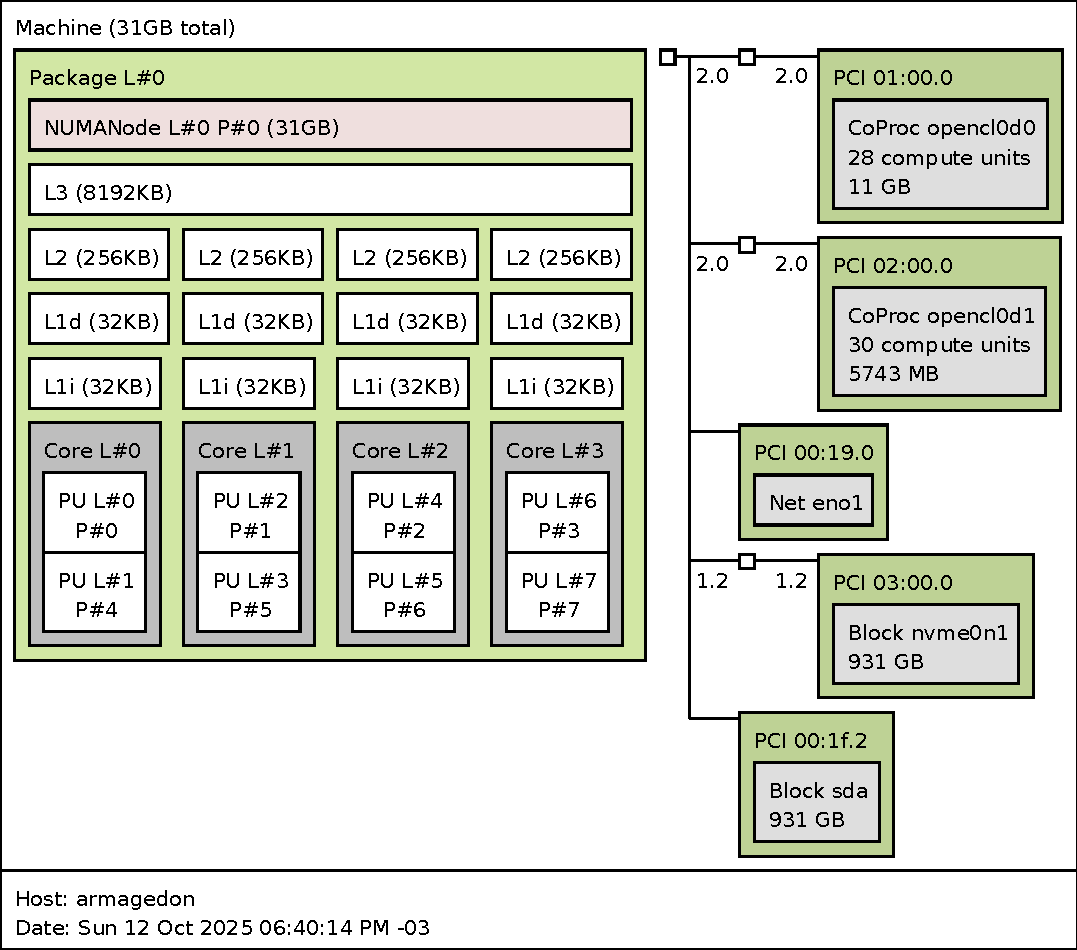
\includegraphics[scale=0.7]{figuras/architecture.pdf}
	\fonte{}
	\addcontentsline{loge}{figure}{\protect\numberline{\thefigure}Especificação do computador utilizado em testes.}
\end{figure}

\section{Conjunto de \textit{Benchmarks}}\label{sec:benchmark}

A seleção das aplicações que compõem o conjunto de benchmarks teve como principais critérios a tolerância a erros e a estrutura do algoritmo. Buscou-se contemplar uma gama ampla de domínios, incluindo \textit{machine learning}, álgebra linear, modelos estatísticos e multimídia. Outro objetivo foi preservar ao máximo o código original durante a inserção das regiões paralelizadas, evitando modificações significativas na implementação. Parte dessas aplicações foi obtida a partir do conjunto PolyBench~\cite{polybench}.

\subsection{2MM}\label{subsec:2mm}

2mm~\cite{polybench} é uma aplicação que realiza a multiplicação sequencial de duas matrizes, utilizando três matrizes distintas: $A$, $B$ e $C$. O processo de execução é ilustrado pelas equações \autoref{eq:dot_matrix_a} e \autoref{eq:dot_matrix_b}.

\begin{equation}
	\label{eq:dot_matrix_a}
	D = A \cdot B
\end{equation}

\begin{equation}
	\label{eq:dot_matrix_b}
	E = C \cdot D
\end{equation}

O algoritmo de multiplicação de matrizes empregado segue o padrão clássico~\cite{axler2015} descrito na \autoref{eq:multi_matrix}, que mostra a multiplicação de duas matrizes 2x2, representando o processo de somas e multiplicações sequenciais. A implementação utilizada pelo \textit{benchmark} é apresentada no \autoref{alg:mul_matrix}.

\begin{equation}
	\label{eq:multi_matrix}
	\begin{bmatrix}
		a_1 & a_2 \\
		a_3 & a_4
	\end{bmatrix}
	\cdot
	\begin{bmatrix}
		b_1 & b_2 \\
		b_3 & b_4
	\end{bmatrix}
	=
	\begin{bmatrix}
		a_1b_1 + a_2b_3 & a_1b_2 + a_2b_4 \\
		a_3b_1 + a_4b_3 & a_3b_2 + a_4b_4
	\end{bmatrix}
\end{equation}

\begin{algorithm}[htb]
	\caption{Multiplicação de matrizes}
	\label{alg:mul_matrix}
	\hrule
	\begin{algorithmic}[1]
		\REQUIRE Matrizes $A$ de tamanho $n \times m$, $B$ de tamanho $m \times p$, $C$ de tamanho $n \times p$
		\FOR{$i = 0$ até $n$}
		\FOR{$j = 0$ até $p$}
		\FOR{$k = 0$ até $m$}
		\STATE $C[i][j] = C[i][j] + A[i][k] \cdot B[k][j]$
		\ENDFOR
		\ENDFOR
		\ENDFOR
	\end{algorithmic}
	\hrule
	\fonte{\citet{polybench}}
\end{algorithm}

Nesta aplicação, ambas as multiplicações são executadas em sequência, conforme as equações \autoref{eq:dot_matrix_a} e \autoref{eq:dot_matrix_b}. Para reduzir o \textit{overhead}, optou-se por utilizar uma única região paralela que abrange ambas multiplicações. Junto a paralelização foi empregado a técnica de \textit{loop tiling}~\cite{bakos2016}. Essa técnica consiste em dividir o espaço de iteração em blocos menores, \textit{tiles}, de modo que cada bloco seja completamente processado antes de avançar para o próximo. Diferentemente da iteração convencional, que percorre toda uma dimensão por vez, no \textit{tiling} os acessos a memória são reorganizados para melhorar a localidade espacial e temporal.

O principal benefício dessa otimização está no uso mais eficiente da \textit{cache}. Idealmente, cada bloco deve ser dimensionado de forma que seus dados caibam inteiramente na \textit{cache}, permitindo que todo o bloco seja carregado e processado de uma só vez. Dessa forma, reduz-se o número de acessos à memória principal e evita-se o recarregamento de dados já utilizados, aumentando o desempenho da aplicação~\cite{bakos2016}. O \autoref{alg:tiling} apresenta o pseudocódigo de implementação dessa técnica na multiplicação de matrizes.

\begin{algorithm}[htb]
	\caption{Multiplicação de matrizes com \textit{loop tiling}}
	\label{alg:tiling}
	\hrule
	\begin{algorithmic}[1]
		\REQUIRE Matrizes $A$, $B$ e $C$ de tamanho $n \times n$
		\REQUIRE Tamanho do bloco $bs$
		\FOR{$ii = 0$ até $n$, em passos de $bs$}
		\FOR{$kk = 0$ até $n$, em passos de $bs$}
		\FOR{$i = ii$ até $\min(ii + bs, n)$}
		\FOR{$k = kk$ até $\min(kk + bs, n)$}
		\STATE $a\_val \gets A[i][k]$
		\FOR{$j = 0$ até $n$}
		\STATE $C[i][j] \gets C[i][j] + a\_val \times B[k][j]$
		\ENDFOR
		\ENDFOR
		\ENDFOR
		\ENDFOR
		\ENDFOR
	\end{algorithmic}
	\hrule
	\fonte{}
\end{algorithm}

\subsection{Correlação}\label{subsec:correlation}

T~\cite{morettin2010}.

A correlação é uma medida estatística que expressa o grau de associação entre duas variáveis. Quando há correlação entre duas variáveis, isso indica que mudanças em uma delas tendem estar relacionadas a mudanças na outra.

A correlação pode ser positiva quando, ambas as variáveis aumentam ou diminuem juntas, ou negativa, quando uma variável aumenta enquanto a outra diminui. O valor da correlação varia de -1 a 1. Valores próximos de 1 indicam uma forte correlação positiva, enquanto valores próximos de -1, uma forte correlação negativa e valores próximos de 0 indicam uma fraca ou nenhuma correlação. A \autoref{fig:correlation}, ilustra esses três tipos de correlação, nos quais é possível observar visualmente o comportamento das variáveis em cada caso.

A fórmula comumente utilizada para calcular a correlação é chamada de \textit{Pearson Correlation Formula}, apresentada na \autoref{eq:correlation}. Nessa equação, $x$ e $y$ representam os valores das variáveis, enquanto $m_x$ e $m_y$ correspondem as suas repectivas médias.

\begin{equation}
	\label{eq:correlation}
	r = \frac{\sum(x - m_x)(y - m_y)}{\sqrt{\sum(x-m_x)^2 \sum(y - m_y)^2}}
\end{equation}

O cálculo da correlação entre as diferentes variáveis está apresentado na \autoref{tab:correlation}. Uma importante propriedade desse cálculo, está no fato de que ela é uma matriz simétrica, isto é, os valores localizados na parte inferior da matriz são iguais aos da parte superior em relação a diagonal principal. Essa diagnoal principal contém valores iguais a $1.0$, correspondentes a autocorrelação perfeita de cada variável. Essa simetria permite otimizar o cálculo, reduzindo o número de iterações, uma vez que é suficiente computar os coeficientes para apenas uma das metades da matriz.

\begin{table}[htb]
	\centering
	\begin{tabular}{|c|c|c|c|c|}
		\hline
		           & \textbf{a} & \textbf{b} & \textbf{c} & \textbf{d} \\
		\hline
		\textbf{a} & 1.0        & ab         & ac         & ad         \\
		\hline
		\textbf{b} & ab         & 1.0        & bc         & bd         \\
		\hline
		\textbf{c} & ac         & bc         & 1.0        & cd         \\
		\hline
		\textbf{d} & ad         & bd         & cd         & 1.0        \\
		\hline
	\end{tabular}
	\caption{Representação da correlação entre as diferentes variáveis}
	\fonte{}
	\label{tab:correlation}
\end{table}

\subsection{Deriche}\label{subsec:deriche}

\subsection{Jacobi 2D}\label{subsec:jacobi2d}

Em análise numérica, o método de Jacobi é um algoritmo iterativo utilizado para resolver sistemas de equações lineares do tipo $Ax = b$. Para que o método funcione adequadamente, o sistema deve atender a algumas condições específicas:

\begin{itemize}
	\item \textbf{Matriz quadrada:} A matriz dos coeficientes deve ser quadrada, ou seja, possuir o mesmo número de linhas e colunas;
	\item \textbf{Sistema linear:} O método aplica-se exclusivamente a sistemas lineares, ou seja, não deve haver termos como multiplicação entre variáveis ($xy$), potências superiores a 1 ($x^2$, $y^3$, etc.), nem funções não lineares, como seno, cosseno ou exponenciais ($e^x$);
	\item \textbf{Diagonal dominante:} Embora não seja uma exigência absoluta, a presença de dominância diagonal na matriz dos coeficientes é altamente recomendada, pois contribui para a garantia de convergência do método. Em sua ausência, o processo iterativo pode apresentar convergência lenta ou até mesmo não convergir.
\end{itemize}

Esse algoritmo foi selecionado como parte do conjunto de \textit{benchmarks} adotados neste trabalho por sua natureza iterativa e previsível em termos de comportamento computacional. O processo inicia-se com a atribuição de valores iniciais arbitrários ao vetor $x$. Em seguida, realiza-se uma iteração para calcular uma nova estimativa da solução, com base exclusivamente nos valores da iteração anterior. Esses novos valores são utilizados como entrada para a próxima iteração. Esse procedimento é repetido até que a diferença entre iterações consecutivas seja inferior a um limiar de tolerância pré-definido, indicando a convergência para uma solução estável.

O Jacobi 2D é uma aplicação do método de Jacobi adaptado para problemas discretizados em duas dimensões. Sua implementação se baseia em um algoritmo de estêncil, no qual cada ponto de uma malha bidimensional é atualizado com base na média artimética dos seus quatro vizinhos imediatos (acima, abaixo, esquerda e a direita), como mostra a \autoref{fig:jacobi2d}. Após um número suficiente de iterações, a malha converge para uma configuração estável que representa uma aproximação da solução contínua do problema.

\subsection{K-means}\label{subsec:kmeans}

O algoritmo K-means é uma técnica de agrupamento, que tem como objetivo particionar um conjunto de dados em $k$ grupos, de forma que os dados dentro de um mesmo grupo de modo que eles sejam semelhantes entre si.

A ideia central do algoritmo consiste em definir inicialmente $k$ centróides, que são pontos de referência no espaço de amostragem. Em seguida, cada ponto de dado é associado ao centróide mais próximo, com base em uma medidade de distância, usualmente a distância euclidiana. Após essa etapa de atribuição, o algoritmo calcula a média dos pontos atribuídos a cada grupo e atualiza a posição dos centróides com base nesses valores.

Esse processo é repetido iterativamente, os dados são reagrupados com base nos novos centróides e os centróides são novamente recalculados. O algoritmo continua até atingir um critério de parada, que pode ser um número fixo de iterações ou a estabilização dos centróides. Durante a execuçõa, o algoritmo também avalia a variância, uma medida que indica o quão disperso os pontos estão em relação ao seu centróide. Quanto menor essa variância, mais compactos são os grupos formados. Embora o objetivo não seja minimizar a variância até zero, uma variância excessivamente alta pode indicar que os dados não estão sendo agrupados de maneira eficiente.

\subsection{Mandelbrot}\label{subsec:mandelbrot}

Mandelbrot é um conjunto de duas dimensções, definida no conjunto dos números complexos. Ele é construído a partir da iteração da função apresentada na \autoref{eq:mandelbrot}, onde $z$ e $c$ são números complexos, com $c$ constante para cada ponto avaliado e a condição inicial $z_0 = 0$.

\begin{equation}
	\label{eq:mandelbrot}
	z_{n + 1} = z_n^{2} + c
\end{equation}

Nem todos os valores de $c$ pertencem ao conjunto de Mandelbrot. Um número complexo $c$ faz parte do conjunto se, ao aplicar a equação iterativamente, a sequência gerada não divergir, ou seja, os valores de $z_n$ permanencem no limite determinado mesmo após várias iterações. Na prática, considere-se que a sequência diverge quando $z_n > 2$, pois se isso continuará crescendo indefinidamente.

Para gerar a representação visual do conjunto Mandelbrot, mapeia-se cada pixel de uma imagem para um número complexo $c$. As regiões do plano onde $c$ pertence ao conjunto são então representadas visualmente.

Os valores de $c$ são escolhidos em um retângulo do plano complexo, com a parte real no intervalo $[-2, 1]$ e a parte imaginária em $[-1.5, 1.5]$. A conversão das coordenadas dos pixels para coordenadas no plano complexo é feita pelas equações \autoref{eq:mandelbrot_cx} e \autoref{eq:mandelbrot_cy}, onde $p_x$ e $p_y$ representam as coordenadas do pixel, e $x_{text{min}}$ e $x_{text{max}}$ definem o domínio da parte real, enquanto $y_{text{min}}$ e $y_{text{max}}$ definem o domínio da parte imaginária.

\begin{equation}
	\label{eq:mandelbrot_cx}
	c_x = x_{\text{min}} + \frac{p_x}{\text{largura da imagem}} \cdot (x_{\text{max}} - x_{\text{min}})
\end{equation}

\begin{equation}
	\label{eq:mandelbrot_cy}
	c_y = y_{\text{min}} + \frac{p_y}{\text{altura da imagem}} \cdot (y_{\text{max}} - y_{\text{min}})
\end{equation}

Inserimos os valores $c_x$ e $c_y$, nas iterações do Mandelbrot. Cada ponto da imagem é testado, e se a sequência $z_n$ não divergir após um número máximo de iterações, o pixel correspondente é colorido. A \autoref{fig:mandelbrot} apresenta uma visualização típica do conjutno de Mandelbrot.

\subsection{PI de Monte Carlo}\label{subsec:pi}

O método de Monte Carlo consiste em um conjunto de algoritmos estatísticos que utilizam amostragem aleatória para resolver problemas determinísticos ou estimar valores numérico. Sua principal característica é a geração de entradas aleatórias dentro de um domínio previamente definido, seguido da aplicação de uma regra ou função para computar a saída, cujo resultados são então agregados para formar uma estimativa.

No caso específico da estimativa de $\pi$, o método pode ser aplicado de forma bastante intuitiva. Considere um cículo de raio $r = 1$, inscrito em um quadrado de lado $2$, conforme ilustrado na \autoref{fig:pi_circle}. As áreas do círculo e do quadrado são dadas, respectivamente, pela \autoref{eq:area_circle} e \autoref{eq:area_square}. A razão entre essas duas áreas é apresentado na \autoref{eq:rational_area}. Por fim ao isolarmos o $\pi$, obtemos a \autoref{eq:rational_pi}.

\begin{equation}
	\label{eq:area_circle}
	A_{\text{círculo}} = \pi r^2 = \pi
\end{equation}

\begin{equation}
	\label{eq:area_square}
	A_{\text{quadrado}} = 2 \times 2 = 4
\end{equation}

\begin{equation}
	\label{eq:rational_area}
	\frac{A_{\text{círculo}}}{A_{\text{quadrado}}} = \frac{\pi}{4}
\end{equation}

\begin{equation}
	\label{eq:rational_pi}
	\pi = 4 \times \frac{A_{\text{círculo}}}{A_{\text{quadrado}}}
\end{equation}

A partir disso, é possível aplicar o método de Monte Carlo para estimar o valor de $\pi$. Como o círculo está inscrito no quadrado, o domínio de amostragem é o próprio quadrado. Gera-se então, um grande número de pontos aleatórios dentro do quadrado. Para cada ponto $(x, y)$, calcula-se sua distância até a origem. Se a distância for menor ou igual a 1, o ponto está dentro do círculo.

A estimativa de $\pi$ é obtida pela razão entre o número de pontos que caíram dentro do círculo e o número total de pontos gerados, multiplicada por 4, como mostra a \autoref{eq:pi_monte}.

\begin{equation}
	\label{eq:pi_monte}
	\pi \approx 4 \times \frac{\text{pontos dentro do círculo}}{\text{total de pontos}}
\end{equation}

A \autoref{fig:pi} apresenta uma ilustração desse processo de amostragem e da aproximação de $\pi$.

\section{Análise de Desempenho}\label{sec:desempenho}

\section{Resumo dos Experimentos}\label{sec:resumo_exp}
